\documentclass[preview]{standalone}

\usepackage{amsmath}
\usepackage{amssymb}
\usepackage{stellar}
\usepackage{bettelini}
\usepackage{wrapfig}

\hypersetup{
    colorlinks=true,
    linkcolor=black,
    urlcolor=blue,
    pdftitle={Biologia},
    pdfpagemode=FullScreen,
}

\begin{document}

\title{Biologia}
\id{biologia-evoluzione-vita}
\genpage

\begin{snippetdefinition}{evoluzione-definition}{Evoluzione}
    Si tratta del cambiamento nel tempo della frequenze geniche (livello di varietà coinvolta)
    di una popolazione (entità che evolve).
\end{snippetdefinition}

\begin{snippet}{eoni-storia-terra}
    La storia della Terra è divisa in quattro eoni di tempo geologico:
    \begin{itemize}
        \item \textit{Adeano} (da 4500 a 3800 milioni di anni fa), precede
        la formazione delle rocce più antiche del pianeta;
        \item \textit{Archeano} (da 3800 a 2500 milioni di anni fa);
        \item \textit{Proterozoico} (da 2500 a 500 milioni di anni fa);
        \item \textit{Fanerozoico} (ultimi 500 milioni di anni).
    \end{itemize}
\end{snippet}

\begin{snippet}{eventi-terra-illustration}
    \begin{center}
    \begin{figure}[ht]
        \centering
        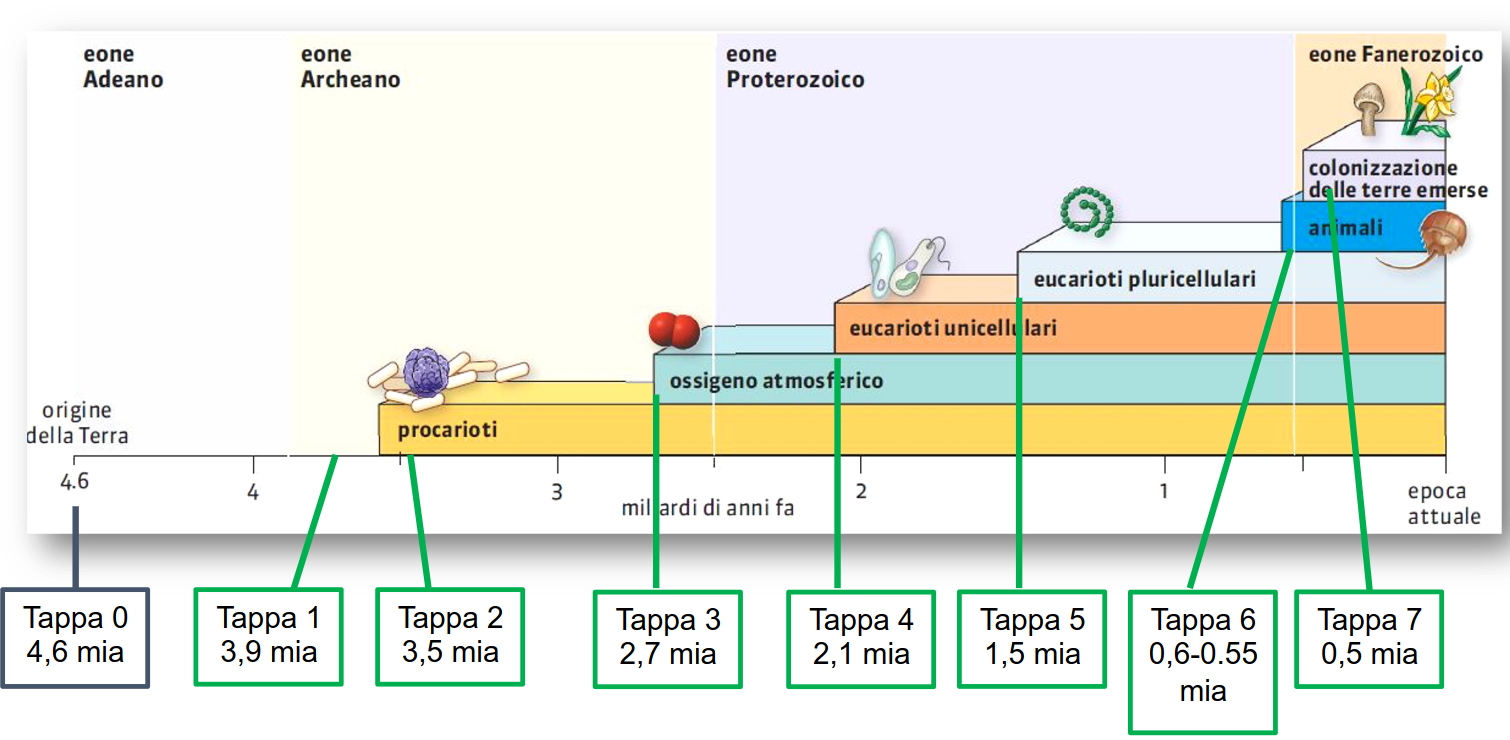
\includegraphics[width=\textwidth]{./resources/eventi-terra.png}
    \end{figure}
    \end{center}
\end{snippet}

\section{Tappa 0: L'origine della Terra primordiale}

\begin{snippet}{7718d4d3-f122-443d-abd9-eed19e7ff943}
    \begin{enumerate}
        \item \textbf{Terra giovane}: materiale fuso, piogge meteoriti, vapore acqueo;
        \item \textbf{Terra dopo 1mia}: raffreddata, solidificata, oceani, atmosfera (diversa!);
        \item \textbf{Condizioni difficili}: piogge di meteoriti, eruzioni vulcaniche, piogge torrenziali, radiazioni UV, etc.
    \end{enumerate}

    Queste condizioni (insieme di componenti e fattori abiotici) hanno
    favorito lo sviluppo della vita, anche se l'esatta formazione della vita rimane un mistero.
\end{snippet}

\section{Tappa 1 - Origine della vita sulla Terra}

\begin{snippet}{b31283cc-d232-466c-8a99-ef7e4cbb9b32}
    Nascono organismi procarioti in acqua (condizioni favorevoli).
    Nello stesso periodo nascono anche i virus.
    Non sappiamo la data effettiva delle prima forme di vita prima di questa data.
\end{snippet}

\section{Tappa 2 - Comparsa della fotosintesi}

\begin{snippetdefinition}{stromatoliti-definition}{Stromatoliti}
    Gli \textit{stromatoliti} sono la prima testimonianza fossile di forme di vita sulla Terra.
    Essi rappresentano la prima apparizione della fotosintesi.
\end{snippetdefinition}

\begin{snippet}{5b19fa42-0c95-4e79-a532-769d98ccc2ef}
    Gli stromatoliti suggeriscono che la vita debba essere originata prima
    poiché la fotosintesi è molto complessa: probabilmente ci sono stati inizialmente
    dei processi più semplici.
    Probabilmente (alcuni) amminoacidi si sono sviluppati spontaneamente dalla materia
    inorganica.
\end{snippet}

\begin{snippet}{tabella-fotosintesi-chemiosintesi}
    $$
\begin{array}{|l|c|c|}
\hline & \text { Fotosintesi } & \text { Chemiosintesi } \\
\hline \begin{array}{l}
\text { Quali spinte? (fonte di } \\
\text { energia come grandezza) }
\end{array} & \text { Luce } & \text { Metano, Acido solfidrico } \\
\hline \begin{array}{l}
\text { Quali cellule sono } \\
\text { implicate? }
\end{array} & \begin{array}{c}
\text { Batteri fotoautotrofe } \\
\text { Vegetali che detengono } \\
\text { l'organello cloroplasto }
\end{array} & \text { Batteri chemioautotrofi } \\
\hline \begin{array}{l}
\text { Quali biomolecole sono } \\
\text { prodotte? }
\end{array} & \begin{array}{c}
\text { Di base lo zucchero, poi le } \\
\text { altre }
\end{array} & \begin{array}{c}
\text { Di base lo zucchero, poi le } \\
\text { altre }
\end{array} \\
\hline \begin{array}{l}
\text { Quali sostanze di scarto } \\
\text { sono prodotte? }
\end{array} & \begin{array}{c}
\text { Ossigeno }
\end{array} & \begin{array}{c}
\text { Zolfo e acqua }
\end{array} \\
\hline
\end{array}
$$
\end{snippet}

\section{Tappa 3 - Comparsa del diossigeno}

\begin{snippet}{9cd4df9a-2262-4926-9278-4800513d7209}
    L'aumento atmosferico aumenta attorno a tutto il pianeta, riempiendo le acquee
    di ossigeno.
    Questo cambiamento avviene dopo diverse centinaia di milioni di anni.
    Infatti, la fotosintesi prima era la fotosintesi
    \textit{anossigenica}, ossia senza ossigeno.
\end{snippet}

\begin{snippet}{differenza-fra-fotosintesi}
    \textbf{Fotosintesi ossigenica:}
    \[ 6\text{CO}_2 + 12\text{H}_2\text{O} + \text{light energy} \longrightarrow \text{C}_6\text{H}_12\text{O}_6 + 6\text{O}_2 + 6\text{H}_2\text{O} \]
    \textbf{Fotosintesi anossigenica:}
    \[ \text{CO}_2 + 2\text{H}_2\text{O} + \text{light energy} \longrightarrow [\text{CH}_2\text{O}] + 2\text{A} + \text{H}_2\text{O} \]
\end{snippet}

\begin{snippet}{3320f23c-8c55-4334-9b23-4e32147ae449}
    Dopo l'aumento di diossigeno nell'atmosfera, molti organismi sono morti
    per la sua tossicità - solo alcuni (quelli mutati) sono rimasti e hanno continuato a riprodursi in
    maniera asessuale. Da questi processi nasce la respirazione cellulare, e
    quest'ultimi hanno prosperato.
\end{snippet}

\section{Tappa 4 - Comparsa degli eucarioti}

\begin{snippet}{nascita-cellule-eucarioti}
    Le cellule eucarioti nascono da una cellula procariote
    più grande che ha assorbito una o più cellule procariote più piccole senza digerirle.
    Le cellule procariote assorbite hanno continuato a vivere all'interno della cellula ospite più grande, in una sorta di simbiosi mutualistica, dove entrambe le parti traggono beneficio dalla relazione.
    Nel corso del tempo, le cellule assorbite si sono specializzate in specifiche funzioni all'interno della cellula ospite. Ad esempio, alcune potrebbero essere diventate organelli come i mitocondri, responsabili della produzione di energia, e i cloroplasti, responsabili della fotosintesi nelle piante.
    Le cellule ospiti e i loro organelli si sono coevoluti, adattandosi l'una all'altra e migliorando la loro efficienza metabolica e funzionale.
\end{snippet}

\section{Tappa 5 - Comparsa eucarioti pluricellulari}

\begin{snippet}{250f6657-ab1b-4dac-a67b-162d5032a761}
    I più antichi fossili di questo gruppo appartengono a delle
    piccole alghe risalenti a 1.2 mia anni fa.
\end{snippet}

\section{Tappa 6 - Animali e esplosione del Cambriano}

\begin{snippet}{esplosione-cambriano}
    Comparsa degli animali (0.6 mia): corpo molle (Fauna di Ediacara)
    Esplosione del Cambriano (0.55 mia): enorme aumento della diversità
    degli animali, comparsa di quasi tutti i phyla degli animali di oggi.
\end{snippet}

\section{Tappa 7 - Alla conquista delle terre emerse}

\begin{snippet}{conquista-terre}
    Inizio della colonizzazione delle terre emerse da parte
    di funghi, piante e animali.
\end{snippet}

\end{document}